% Use class option [extendedabs] to prepare the 1-page extended abstract.
\documentclass[extendedabs]{bmvc2k}
\usepackage[colorlinks = true,
            linkcolor = blue,
            urlcolor  = blue,
            citecolor = blue,
            anchorcolor = blue]{hyperref}
\usepackage{bm}
\usepackage{mathrsfs}
\usepackage{mathtools}
 \usepackage{nccmath}
\usepackage{bbold}
\newcommand\ii{{\mathrm{i}}}
\DeclareMathOperator{\Tr}{{Tr}}
\newcommand{\Com}[2]{\left[{#1},{#2}\right]}
\DeclarePairedDelimiter{\diagfences}{(}{)}
\newcommand{\diag}{\operatorname{diag}\diagfences}

% Document starts here
\begin{document}

\title{Many Body Quantum Kinetics in the Phase Space:\\
Simulating spin dynamics by the BBGKY trajectories of sampled phase points}
\addauthor{
Analabha Roy$^1$,$^2$
}{}{1}
\addinstitution{
$^1$National Institute for Theoretical Physics, Stellenbosch University, Stellenbosch $7600$, South Africa \\ 
$^2$Department of Physics, The University of Burdwan, Barddhaman $713104$, India
}
 
\maketitle

% Extended abstract begins here.  In a one-page document, there is
% little need for section headers, but you may use \section etc if you
% wish.

\noindent
A novel method for simulating the quantum many body dynamics of discrete spins is presented. This method extends the Truncated Wigner Approximation in the phase space
spanned by discrete spin eigenvalues with the quantum kinetics of $2$- point correlations obtained from the Bogoliubov-Born-Green-Kirkwood-Yvon (BBGKY) hierarchy. Going to higher orders of the BBGKY hierarchy allows for a systematic refinement of the method. Quantum correlations are treated through both, the Wigner function sampling and the BBGKY evolution. Thus, the method is highly accurate for long times, and is especially well suited for long range interactions, higher dimensional problems, and strongly correlated systems. The efficacy of this method is demonstrated by comparing with exact results as well as methods involving Matrix Product States. Current applications of this method involve the  computation of spin-squeezing in a two-dimensional lattice with power-law interactions and a transverse field, as well as a simulation of  photon-mediated co-operative effects in the quantum dynamics of a large cloud of atoms.

In the Truncated Wigner Approximation (TWA), the exact dynamics of a quantum system with Hamiltonian $\hat{H}$ and density operator $\hat{\rho}$ is written in the phase space spanned by $(q,p)$, the eigenvalues of the canonically conjugate position-momentum operators $(\hat{q},\hat{p})$, as
\begin{equation}
\label{eq:twa}
\partial_t W(q,p) = \ii \bigg\{W(q,p),H_C(q,p)\bigg\}_{M.B}.
\end{equation}
Here, the Wigner function $W(q,p)$ is defined as the Weyl symbol of the density matrix~\cite{Polkovnikov10}, \textit{viz.}, $W(q,p) \equiv \Tr{\left\{\hat{\rho} \exp{\left[i\left(p\hat{q}-q\hat{p}\right) \right]}\right\}}$, the Moyal Bracket on the RHS of eqn~\ref{eq:twa} is defined as $\left\{W(q,p),H_C(q,p)\right\}_{M.B}\equiv W(q,p)
\{2\sin[$\\
$\overleftarrow{\partial_p}\overrightarrow{\partial_q}-\overleftarrow{\partial_q}\overrightarrow{\partial_p}]\}H_C(q,p)$, and $H_C$, the Weyl symbol of the Hamiltonian, is just the classical Hamiltonian in the phase space, provided that the quantum Hamiltonian is normal-ordered in $(\hat{q},\hat{p})$. The TWA involves truncating the Moyal Bracket expansion of the $\sin$-term in eqn~\ref{eq:twa} to the lowest order, yielding the Poisson bracket, \textit{i.e.}, the classical dynamics of the Wigner function $W(q,p)$. This dynamics is simulated by a Monte-Carlo sampling of the phase points, biased by the quasi-probability distribution $W(q,p)$. The dynamics of an observable $\hat{\Omega}$ is approximated from that of its classically evolving Weyl symbol in the TWA, averaged over all chosen sample points.

The TWA can be discretized to simulate the dynamics of spin-$1/2$ particles~\cite{Wootters87}. In the Discrete Truncated Wigner Approximation (DTWA), phase-point operators $\hat{A}_\alpha\equiv \frac{1}{2}(\mathbb{1}+\bm{r}_\alpha\cdot\bm{\sigma})$ can be defined for $4$ discrete phase points (indexed by $\alpha$) for each spin. Here, the choice of $3-$vectors $\bm{r}_\alpha$ denotes a particular sampling scheme, and the choices are made so as to satisfy projection properties that are analogous to those of the operators $\exp{\left[i\left(p\hat{q}-q\hat{p}\right)\right]}$ in the continuous TWA~\cite{Schachenmaye15}. Also, $\bm{\sigma}\equiv(\sigma^x, \sigma^y,\sigma^z)$, the vector of Pauli matrices. The discrete Wigner function is defined for each spin as a collection of $4$ values  $w_\alpha\equiv \Tr{[\hat{\rho} \hat{A}_{\alpha}]}$ for each single-spin phase point $\alpha$~\cite{Schachenmaye15}. A particular example of the Wigner function for a spin, fully polarized in $x$, is shown as a table of $4-$values in fig~\ref{f:wigner:init}. If the initial many body state in an $N-$spin system is an un-entangled product state, then the discrete Wigner function of the full system can be written as a product of $w_\alpha$s for each spin, allowing for the expansion of the full many body density operator
\begin{equation}
\hat{\rho}_0\equiv \hat{\rho}(t=0) = \displaystyle\sum_{\alpha_1,\dots,\alpha_N} w_{\alpha_1}\dots w_{\alpha_N}\; \hat{A}_{\alpha_1}\otimes \dots \otimes \hat{A}_{\alpha_N}.
\end{equation}
Here, $\hat{A}_{\alpha_1}\otimes \dots \otimes \hat{A}_{\alpha_N} = \mathscr{A}^{\alpha_1\dots\alpha_N}(t=0)$, is a single many-body phase point constructed from the individual sampled phase points $\alpha_1\dots\alpha_N$. The full many body dynamics of the system can be formulated from the exact dynamics of all phase point operators $\mathscr{A}^{\alpha_1\dots\alpha_N}(t)$~\cite{Pucci16}. This is approximated by a finite sample of $n_t$ phase points (biased by the quasi-probabilities $w_\alpha$), followed by the classical evolution of the spins $s_i$ using the classical spin Hamiltonian $H_c$, the Weyl transform of the quantum spin Hamiltonian.

Comparison of the DTWA with exact and MPS-DMRG solutions for long range spin systems have yielded relatively good results for single spin observables such as $\langle \sigma^\mu_i(t)\rangle$, but poorer results for $2-$spin correlations, such as $\langle \sigma^\mu_i(t) \sigma^\nu_j(t)\rangle$, at long times~\cite{Schachenmaye15}. While correlations in the initial state are reflected in the Wigner function and the subsequent sampling, individual phase points from the sample evolve classically in mean-field trajectories. Therefore, DTWA incorporates quantum correlations only on the level of the initial state and accounts for them only for very short times~\cite{Pucci16}. This necessitates systematic refinements of the DTWA by recasting the exact dynamics of the sampled phase points as a BBGKY hierarchy~\cite{Pucci16}. The hierarchy builds the exact Liouville dynamics of a many body system such that the dynamics of $n-$spin correlations, $\langle \sigma^{\mu_1}_1(t) \sigma^{\mu_2}_2(t)\dots\sigma^{\mu_n}_n(t)\rangle$, are  coupled to $(n+1)-$particle correlations, $\langle \sigma^{\mu_1}_1(t) \sigma^{\mu_2}_2(t)\dots\sigma^{\mu_{n+1}}_{n+1}(t)\rangle$, thus
forming a coupled chain of equations.This allows for coupling mean field classical dynamics of single - point operators obtained from DTWA to the semi-quantal dynamics of local correlations. Truncating out third  and higher order connected correlations yield better approximations for the dynamics of each Wigner-sampled phase point, especially in strongly correlated systems. The BBGKY hierarchy also makes this approach highly conducive to the study of long range interactions.

The method described above is illustrated by applying it to a generic $N-$body Hamiltonian with $2-$body interactions,
\begin{equation}\label{eq:hgen}
H_{1\dotsc N} = \sum^N_i H_i + \sum^N_{i<j}H_{ij}.
\end{equation}
The exact  Liouville-von Neumann dynamics of the many body phase point operators,
\begin{equation}\label{eq:vneqdwa}
\ii\partial_t \mathscr{A}^{\alpha_1\dots\alpha_N} = \Com{H}{\mathscr{A}^{\alpha_1\dots\alpha_N}},
\end{equation}
is recasted by taking partial traces $\Tr_{\not{\,i}}$, $\Tr_{\not{\,i}\not{\,j}}$, \dots. Thus, the BBGKY hierarchy of $N$ coupled differential equations is obtained in terms of reduced phase point operators, 
\begin{subequations}
\begin{align}
\ii\partial_t \mathscr{A}_i=&\Com{H_i}{\mathscr{A}_i}+\sum^N_{k\neq i}\Tr\Com{H_{ik}}{\mathscr{A}_{ik}}\label{e:1st_order_app1}\\
\ii\partial_t \mathscr{A}_{ij}=&\Com{H_i+H_j+H_{ij}}{\mathscr{A}_{ij}}\nonumber\\
&+\sum^N_{k\neq i,j}\Tr_k\Com{H_{ik}+H_{jk}}{\mathscr{A}_{ijk}},
\label{e:2nd_order_app1}
\end{align}
\end{subequations}
where only the first two equations of the BBGKY hierarchy are shown. Here, $\mathscr{A}_i\equiv \Tr_{\not{\,i}}{\big[\mathscr{A}^{\alpha_1\dots\alpha_N}\big]}$, $\mathscr{A}_{ij}\equiv \Tr_{\not{\,i}\not{\,j}}{\big[\mathscr{A}^{\alpha_1\dots\alpha_N}\big]}$, etc. Inserting cluster expansions,
\begin{subequations}
\begin{align}
\mathscr{A}_{ij}&=\mathscr{A}_i \mathscr{A}_j+\mathscr{C}_{ij},\label{e:cluster1}\\
\mathscr{A}_{ijk}&=\mathscr{A}_i \mathscr{A}_j \mathscr{A}_k + \mathscr{A}_i \mathscr{C}_{jk} + \mathscr{A}_j \mathscr{C}_{ik} + \mathscr{A}_k \mathscr{C}_{ij} + \mathscr{C}_{ijk},\label{e:cluster2}
\end{align}
\end{subequations}
and similarly for higher orders, into eqns~\ref{e:1st_order_app1} and~\ref*{e:2nd_order_app1} yields
\begin{subequations}
\begin{align}
\ii\partial_t \mathscr{A}_i=&\Com{H_i}{\mathscr{A}_i}+\sum_{k\neq i}\Tr\Com{H_{ik}}{\mathscr{C}_{ik}+\mathscr{A}_i \mathscr{A}_k}\label{e:1st_order}\\
\ii\partial_t \mathscr{C}_{ij}=&\Com{H_i+H_j+H_{i\not{\,j}}^\text{H}+H_{j\not{\,i}}^\text{H}}{\mathscr{C}_{ij}}+\Com{H_{ij}}{\mathscr{C}_{ij}+\mathscr{A}_i \mathscr{A}_j}\nonumber\\
&+\sum_{k\neq i,j}\left(\Tr_k\Com{H_{ik}}{\mathscr{A}_i \mathscr{C}_{jk}}+\Tr_k\Com{H_{jk}}{\mathscr{A}_j \mathscr{C}_{ik}}\right)\nonumber\\
&-\mathscr{A}_i\Tr_i\Com{H_{ij}}{\mathscr{C}_{ij}+\mathscr{A}_i \mathscr{A}_j}\nonumber\\
&-\mathscr{A}_j\Tr_j\Com{H_{ij}}{\mathscr{C}_{ij}+\mathscr{A}_i \mathscr{A}_j},\label{e:2nd_order}
\end{align}
\end{subequations}
\begin{figure}[bht!]\centering
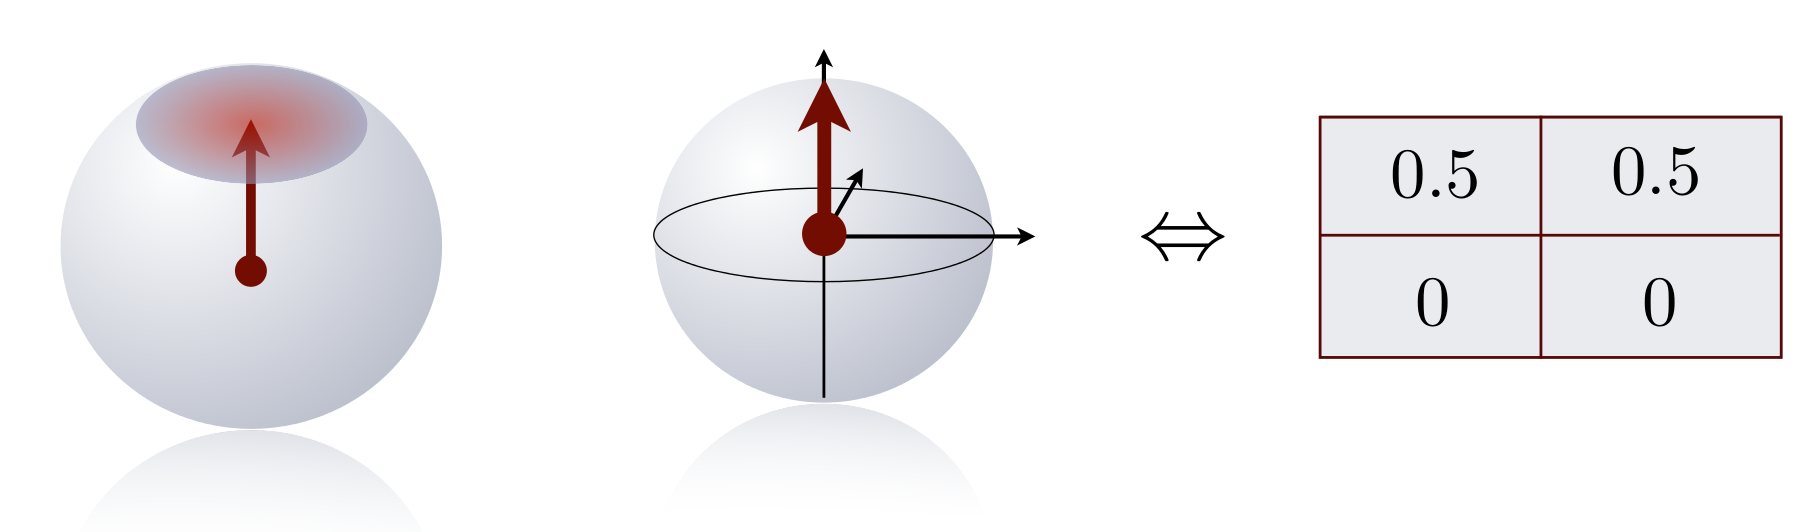
\includegraphics[width=\linewidth]{./images/fig1.jpg}
\caption{\label{f:wigner:init}Schematic diagram illustrating the initial state (for a single spin) used to evolve the Hamiltonian in eq~\ref{eq:curieweiss} by DTWA augmented with BBGKY. A single spin, fully polarized in $x$, has a density matrix $\hat{\rho} = \frac{1}{2}(\mathbb{1}+\sigma^x)$. Unlike the corresponding classical state polarized in $x$ (red arrow pointing in the vertical direction), the quantum state has non-zero probabilities of being found in the $yz$ plane (shaded region around the classical spin on the unit sphere on the left). The state can be completely represented by a discrete Wigner distribution function consisting of $4-$values as seen in the rightmost table. The values $w_\alpha$ (indexed by $\alpha$ in the text) are computed by evaluating $\Tr{[\hat{\rho}\hat{A}_\alpha]}$ for $4$ phase point operators $\hat{A}_\alpha\equiv \frac{1}{2}(\mathbb{1}+\bm{r}_\alpha\cdot\bm{\sigma})$, with the $\bm{r}_\alpha$ chosen to be $ (1, 1, 1), (-1, -1, 1),
(1, -1, -1)$, and $(-1, 1, -1)$. The values are inserted into the table row-wise from the top left.}
\end{figure}
with the Hartree operator
\begin{equation}
 H_{i\not{\,j}}^\text{H}=\sum_{k\neq i,j}\Tr_k\left(H_{ik} \mathscr{A}_k\right).
\end{equation}
Neglecting the $3-$body correlations $\mathscr{C}_{ijk}$ is expected to be good for intermediate times and sufficiently long-ranged interactions. Improving this scheme systematically by truncating the BBGKY hierarchy at higher order is straightforward, at a numerical cost that scales like $\mathscr{O}\left(N^n\right)$ with truncation order $n$. Neglecting the $2-$spin correlations $\mathscr{C}_{ij}$ in \eqref{e:1st_order}, would recover the time evolution equations used in DTWA.

The dynamics depicted in eqns~\ref*{e:1st_order} and~\ref*{e:2nd_order} can be performed numerically for spin systems by representing the $\mathscr{A}$- and $\mathscr{C}$-operators in the basis of Pauli matrices,
\begin{subequations}
\begin{align}
\mathscr{A}_i &= \tfrac{1}{2}\left(\mathbb{1}_i+\bm{a}_i\cdot\bm{\sigma}_i\right),\label{e:Aexp}\\
\mathscr{C}_{ij} &= \tfrac{1}{4}\sum_{\mu,\nu\in\{x,y,z\}}c_{ij}^{\mu\nu}\sigma_i^\mu\sigma_j^\nu,\label{e:Cexp}
\end{align}
\end{subequations}
for $i\neq j$. Inserting these expansions into the BBGKY equations \eqref{e:1st_order} and \eqref{e:2nd_order}, yields
time evolution equations for the expansion coefficients $a_i^\mu$ and $c_{ij}^{\mu\nu}$; see ref~\cite{Pucci16} for a derivation. This set of $3N(3N-1)/2$ coupled ordinary differential equations is the second main ingredient of the simulation method.

Finally, the expectation values of $1-$ or $2-$spin operators can be approximated by averages over the $n_t$ sampled phase points as shown below.
\begin{subequations}
\begin{align}
\left\langle\sigma_i^\mu\right\rangle =& \sum_{\alpha_1\dots\alpha_N}w_{\alpha_1}\cdots w_{\alpha_N} a_i^\mu \approx \frac{1}{n_t}\sum_{\alpha_1\dots\alpha_N} a_i^\mu,\label{e:1spin}\\
\left\langle\sigma_i^\mu\sigma_j^\nu\right\rangle =& \sum_{\alpha_1\dots\alpha_N}w_{\alpha_1}\cdots w_{\alpha_N} \left(c_{ij}^{\mu\nu}+a_i^\mu a_j^\nu\right)\nonumber\\
\approx& \frac{1}{n_t}\sum_{\alpha_1\dots\alpha_N} \left(c_{ij}^{\mu\nu}+a_i^\mu a_j^\nu\right).\label{e:2spin}
\end{align}
\end{subequations}

The method described above is benchmarked against exact results by applying it to the time-evolution Curie-Weiss-type $N-$spin Hamiltonians
\begin{equation}
\label{eq:curieweiss}
H = \sum_{i\neq j}\bm{\sigma}_i\cdot\overset{\text{\tiny$\bm\leftrightarrow$}}{\bm{J}}_{ij}\cdot\bm{\sigma}_j - \bm{h}\cdot\sum_i \bm{\sigma}_i,
\end{equation}
starting from an initial product state given by the fully $x-$polarized density matrix $\hat{\rho}_0 = 2^{-N}(\mathbb{1}+\sigma^x)^{\otimes\;N}$. In eqn~\ref{eq:curieweiss}, $J$ is a dyadic of coupling constants and $\bm{h}$ is an external field. In the first benchmark, the Hamiltonian is reduced to the long-range Ising chain by setting $\overset{\text{\tiny$\bm\leftrightarrow$}}{\bm{J}}_{ij} =\diag{0,0,-\frac{1}{|i-j|^\alpha}}$ and $\bm{h} = 0$. The exponent $\alpha\geq0$ controls the range of the interactions, and open boundary conditions are used. For the Ising model, exact analytic results are known for the time-evolution of $1-$spin and $2-$spin functions. This method is numerically exact for the Ising model, as shown in~\cite{Pucci16}. 
\begin{figure}\centering
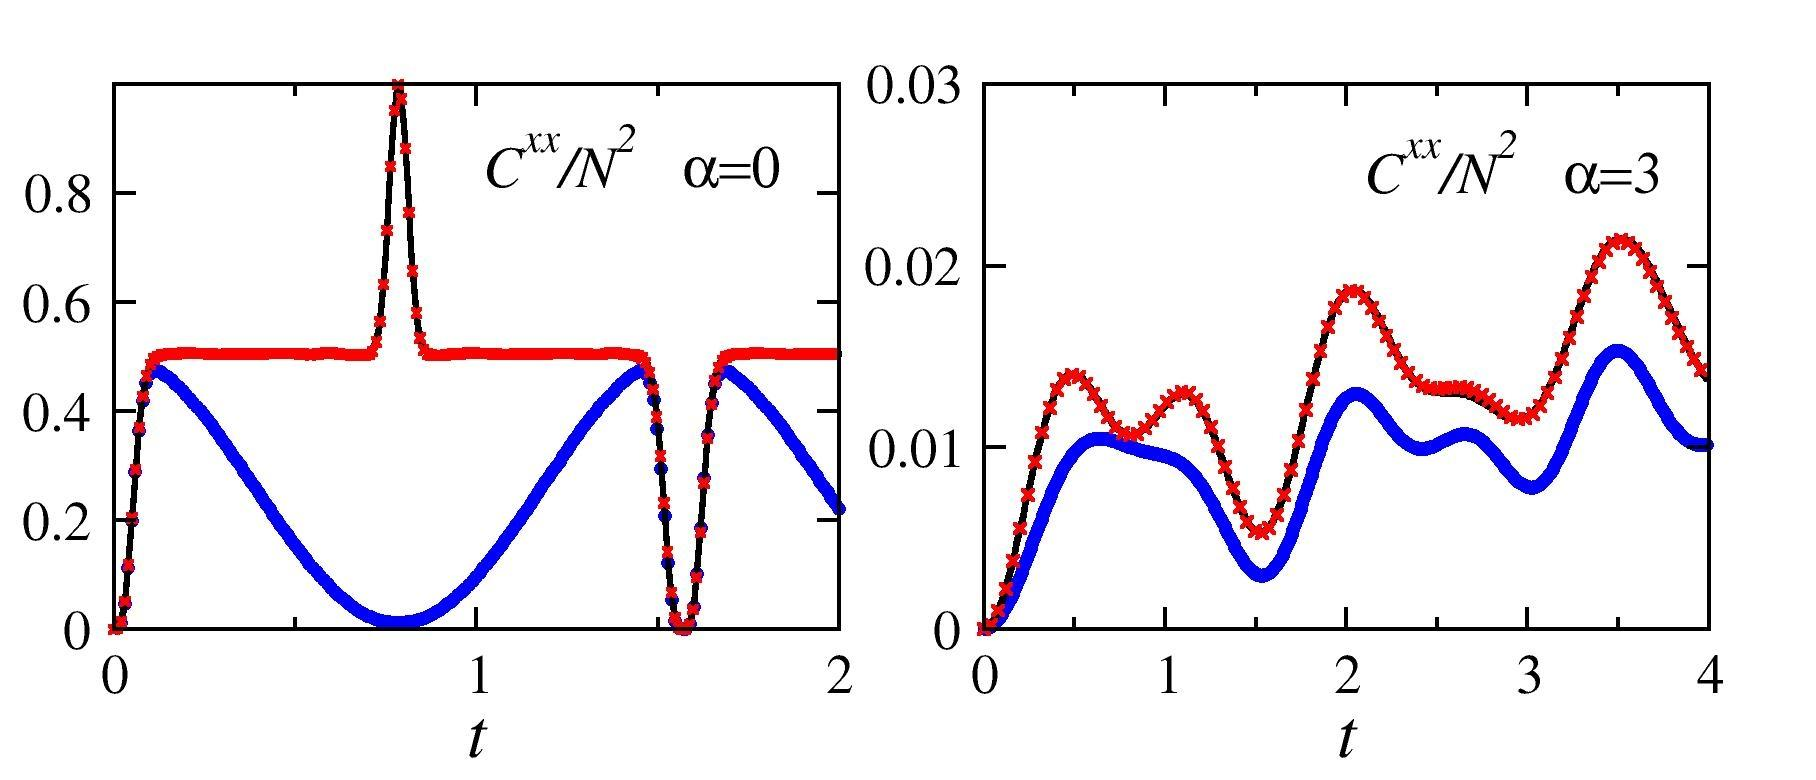
\includegraphics[width=\linewidth]{./images/fig2.jpg}
\caption{\label{f:Ising}%
Time evolution of total connected correlations $C^{xx}$ as defined in eqn~\eqref{e:Cmumu} for a long-range Ising chain of $100$ sites in the absence of a magnetic field and with long-range exponent $\alpha=0$ (left) and $\alpha=3$ (right). As shown analytically in~\cite{Pucci16}, DTWA-BBGKY recovers the exact solution (black) in the limit of an infinite sample. The only error (which is not visible on the scale of the plot) is therefore of a statistical nature due to the finite sample size $n_t=10000$ (red crosses). Using DTWA only (blue dots) shows systematic deviations from the exact result. Reproduced with permission from~\cite{Pucci16}.}%
\end{figure}
A comparison with the method of DTWA, which show deviations from the exact result, is shown in fig~\ref{f:Ising}, where the total connected correlations
\begin{equation}\label{e:Cmumu}
C^{\mu\mu}=\sum_{i,j}\left(\left\langle\sigma_i^\mu\sigma_j^\mu\right\rangle - \left\langle\sigma_i^\mu\right\rangle\left\langle\sigma_j^\mu\right\rangle\right),
\end{equation}
are plotted in time for the exact solution, the DTWA method and the DTWA method augmented with BBGKY.
Further benchmarking has been achieved by reducing the Curie-Weiss Hamiltonian in eqn~\ref{eq:curieweiss} to the XX model by setting 
$\overset{\text{\tiny$\bm\leftrightarrow$}}{\bm{J}}_{ij} =\diag{-\frac{1}{|i-j|^\alpha},-\frac{1}{|i-j|^\alpha},0}$ and $\bm{h} = 0$. This model is particularly instructive, since the fully $x-$polarized state is the classical ground state, and purely classical evolution of the state would not show any dynamics. However, probabilistic sampling via the Wigner function (shown for a single spin-$1/2$ in fig~\ref*{f:wigner:init}) of $x$ and $y$ spins leads to non-trivial dynamics of Monte-Carlo averaged observables in DTWA. Comparison of DTWA with exact DMRG methods for this benchmark, shown in fig~\ref{f:XX}, indicate good agreement for the single-spin observable $S^x(t) = \sum_i \langle \sigma^x_i(t)\rangle$, but poor agreement for $C^{xx}(t)$ (defined in eqn~\ref{e:Cmumu}), as well as the spin-squeezing. Spin-squeezing $\xi$ is defined as the minimum variance of the total spin $\hat{\bm{S}}=\sum_i\bm{\sigma}_i$ in a direction $\bm{n}$ that is perpendicular to the spin expectation $\langle\hat{\bm{S}}\rangle$~\cite{Sorensen01},\textit{i.e.}
\begin{equation}
\label{e:spinsqueezing}
	\xi \equiv \sqrt{N} \min_{\bm{n}\perp\langle\hat{\bm{S}}\rangle}{\frac{\sqrt{\langle
	(\hat{\bm{S}}\cdot\bm{n})^2\rangle-\langle\hat{\bm{S}}\cdot\bm{n}\rangle^2}}{|\langle\hat{\bm{S}}\rangle||\bm{n}|}}.
\end{equation}
This observable was chosen for the benchmark because it encapsulates the dynamics of all possible $2-$spin correlations and witnesses entanglement when it drops below unity~\cite{Sorensen01, Schachenmaye15}. Quantitative agreement of DMRG results with DTWA is dramatically improved for both $C^{xx}(t)$ and $\xi(t)$ when DTWA is augmented with the BBGKY dynamics of phase point operators to second order, as can be seen in fig~\ref{f:XX}. Finally, the DTWA-BBGKY method is neutral with respect to dimensionality, and so works in higher dimensional systems where many exact methods fail. As proof of concept, the spin squeezing $\xi$ of a $2D$ triangular lattice, with $\overset{\text{\tiny$\bm\leftrightarrow$}}{\bm{J}}_{ij}$ obtained from experimental data of a transversely excited  Wigner crystal of ultracold ions in a Penning trap~\cite{Britton12}, is computed and shown in~\cite{Pucci16}.

Generalization of this method to open quantum systems in the Lindblad picture is possible. This allows for modelling experimental decoherence in quantum spin systems, as well as quantum cooperative effects due to light scattering in atomic clouds. Cooperative light-scattering has been simulated on an assembly of $N$ two-level pseudospin$-1/2$ systems, randomly distributed in space, with internal transitions driven by a classical plane-wave  laser~\cite{Pucci17}. The dynamics is described by a set of equations that couple the spin degrees of freedom to the photon field. The photon modes are then traced out, and the rotating wave and Born-Oppenheimer approximations are applied. Thus, for an arbitrary phase point operator $\mathscr{A}$, 
\begin{equation}\label{VNeqdWA}
\ii\partial_t\mathscr{A}=\mathcal{L}\mathscr{A},
\end{equation}
where the Lindblad operator,
\begin{equation}\label{e:Lindblad}
\mathcal{L}=\sum_ i\mathcal{L}_ i+\sum_{ i j}\mathcal{L}_{ i j},
\end{equation}
\begin{figure}\centering
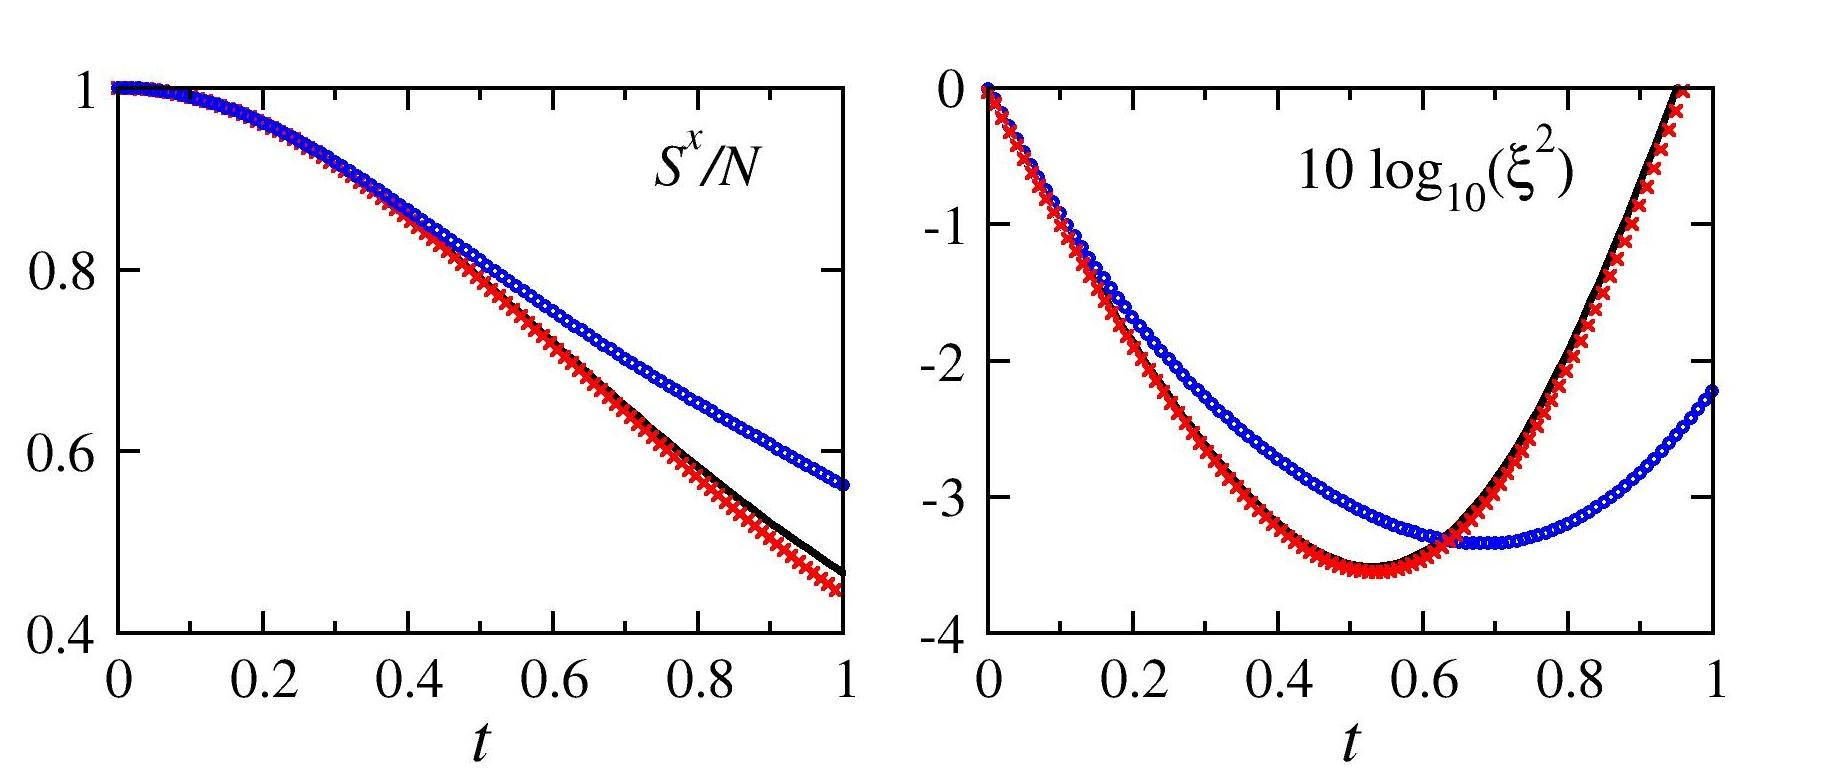
\includegraphics[width=\linewidth]{./images/fig3.jpg}
\caption{\label{f:XX}%
Time evolution of a long-range $XX$ chain of $100$ sites with $\alpha=3$. We compare DMRG results (black line), the method of DTWA (blue dots), and DTWA-BBGKY (red crosses) for sample sizes $n_t=10^5$. Left: Total spin $S^x=\sum_i\sigma_i^x$. Right: Decibel spin squeezing as obtained from \eqref{e:spinsqueezing}, where the results of our method are virtually indistinguishable from the DMRG data. Reproduced with permission from~\cite{Pucci16}.}%
\end{figure}
consists of on-site terms coming from the single-spin Rabi oscillations,
\begin{multline}
\mathcal{L}_ i\mathscr{A}=-\frac{\Delta_0}{2}\Com{\sigma_ i^z}{\mathscr{A}}
+\frac{\Omega_0}{2}\Com{e^{- i\mathbf{k}_0\cdot\mathbf{r}_ i}\sigma_ i^-+e^{ i\mathbf{k}_0\cdot\mathbf{r}_ i}\sigma_ i^+}{\mathscr{A}},
\end{multline}
with detuning $\Delta_0$ and Rabi frequency $\Omega_0$, as well as 
pair interactions 
\begin{multline}\label{e:Lij}
\mathcal{L}_{ i j}\mathscr{A}=\Delta_{ i j}\Com{\sigma_ i^+\sigma_ j^-}{\mathscr{A}}+\\
\ii\gamma_{ij}\left(\sigma_ j^-\mathscr{A}\sigma_ i^+-\tfrac{1}{2}\sigma_ i^+\sigma_ j^-\mathscr{A}-\tfrac{1}{2}\mathscr{A}\sigma_ i^+\sigma_ j^-\right),
\end{multline}
containing the long-range light-mediated spatial coupling between the atoms in the coefficients $\Delta_{ij}+\ii\gamma_{ij}\sim$
$e^{\ii\bm{k}\cdot(\bm{r}_i-\bm{r_j})}\over{\bm{k}\cdot(\bm{r}_i-\bm{r_j})}$, for a laser beam of momentum $\bm{k}$ and atoms at positions $\bm{r}_i$~\cite{Pucci17}. 

The dynamics of the Rabi oscillations manifest spectroscopically as a Mollow triplet due to the Autler-Townes effect. In addition, the light-mediated coupling is expected to induce an asymmetry in the Mollow triplet, as well as  higher order sidebands due to the light-atom coupling as two scatterers interact through their radiation. These are fully cooperative many body effects that scale with the optical thickness. Both phenomena are seen in the DTWA-BBGKY simulations (see fig~\ref{fig:SpecBabies}) when the spectrum is evaluated from the $2-$time $2-$spin correlations
\begin{equation}\label{evol_2r_corr}
\langle\sigma_ i^\mu(t)\sigma_ j^\nu(t+\tau)\rangle=\Tr\left\{V(t+\tau,t)\left[\left(V(t,0)\hat{\rho}_0\right)\sigma_ i^\mu\right]\sigma_ j^\nu\right\},
\end{equation}
where the RHS follows from the quantum regression theorem~\cite{Pucci17}. In eqn~\ref{evol_2r_corr}, the propagator $V$ evolves the density matrix with the exact dynamics in eqn~\ref{e:Lindblad}. In the long-time limit, the correlations can be written in terms of the nonequilibrium steady state density matrix $\hat{\rho}_\text{ss} = \displaystyle\lim_{t\rightarrow\infty} V(t,0)\hat{\rho}_0$ as
\begin{equation}\label{limcorr}
\lim_{t\to\infty}\langle\sigma_ i^a(t)\sigma_ j^b(t+\tau)\rangle=\Tr\left[\sigma_ j^b V(\tau,0)\left(\hat{\rho}_\text{ss}\sigma_ i^a\right)\right].
\end{equation}
The propagation of $\hat{\rho}_\text{ss}\sigma_ i^a$ is approximated by writing it in terms of single-spin phase point operators $\hat{A}_{\alpha_i}$, then using the DTWA-BBGKY method to approximate the Lindblad dynamics of $4N$ (for each phase point) reduced operators, namely, $N$ scalar operators $\mathscr{A}^{(0)}_i = \Tr_i{[\hat{\rho}_\text{ss}]}\hat{A}_{\alpha_i}$, and $3N$ operators $\mathscr{{A}}^{(\mu)}_i = \Tr_i{[(\mathbb{1}+{\sigma^\mu}_i)\hat{\rho}_\text{ss}]}\hat{A}_{\alpha_i}/(1+\Tr{[{\sigma}^\mu_i\hat{\rho}_\text{ss}}])$, to second order in correlations. This yields equations similar in structure eqns~\ref{e:1st_order} and~\ref{e:2nd_order}~\cite{Pucci17}. The resultant spectrum is shown in fig~\ref{fig:SpecBabies}, together with the scaling of the sidebands that appear after the Mollow triplet.

Thus, the DTWA-BBGKY method for simulating the time evolution of quantum spin models is introduced and its efficacy shown for closed many body spin systems, as well as more complex many body interactions. While DTWA-BBGKY is accurate to experimentally accessible timescales, further refinements are necessary for theoretical studies. The prospects of this method are strong, with the possibility of using it to explore universality in the nonequilibrium dynamics of long-range spin systems (such as the Kibble-Zurek mechanism, superluminal correlation dynamics~\cite{Eisert13}, quantum ergodicity, and superradiance) just beyond the horizon.
\begin{figure}
\centering
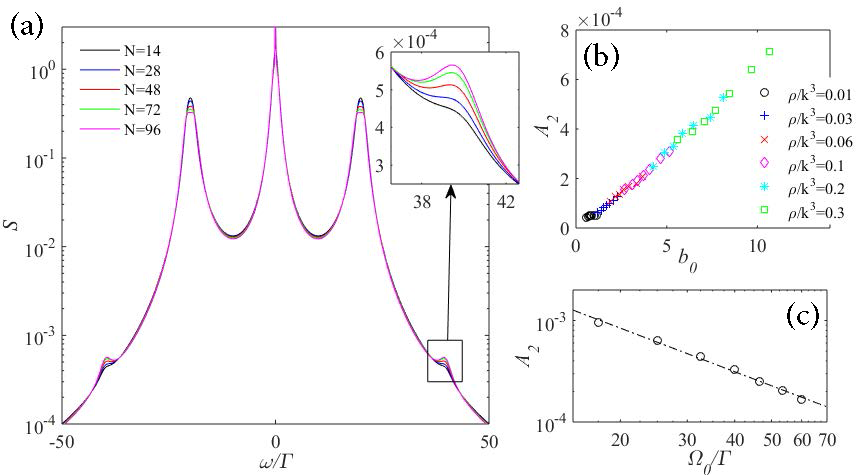
\includegraphics[width=1\linewidth]{./images/fig4.png}
\caption{\label{fig:SpecBabies} (a) Fluorescence spectrum for a cloud of density $\rho/k^3=0.1$ obtained using DTWA-BBGKY. The cloud is driven at $\Omega_0=20\Gamma$ with detuning $\Delta_0=0$, for $N=14-96$ atoms. The inset shows the behaviour of the peaks at $\omega\approx2\Omega_0$. The amplitude of the additional Mollow sidebands can be seen as a function of (b) the optical thickness $b_0$ for different densities ($\Omega=20\Gamma$, $N=72$ and $\Delta_0=0$) and (c) of the Rabi frequency ($\rho/k^3=0.1$, $N=72$ and $\Delta_0=0$). The dash-dotted line in (c) refers to a power-law fit ($A_2\approx 0.06(\Omega/\Gamma)^{-1.4}$). Reproduced with permission from~\cite{Pucci17}.}
\end{figure}
\section*{References}
\bibliography{conference_ext_abstract}
\end{document}
